\notechapter{N-20260325}{Extrema of Two-Variable Functions and the Hessian Test}

\section{Local extrema}

Let \(f:G\subseteq\mathbb R^2\to\mathbb R\).  A point \(P_0\in G\) is a \vocab{local maximum} if there is a neighborhood \(U\) of \(P_0\) such that
\[
  f(P)\le f(P_0)\qquad(P\in U\cap G).
\]
It is a \vocab{local minimum} if the inequality is reversed.  If the inequality is strict for all nearby \(P\ne P_0\), the extremum is strict.

The word "local" matters.  A point can be best among nearby points without being best on the whole domain.

\section{First-order necessary condition}

\begin{theorem}[Fermat theorem in several variables]
If \(f\) is differentiable at an interior point \(P_0\in G\) and \(P_0\) is a local extremum, then
\[
  \nabla f(P_0)=0.
\]
\end{theorem}

\begin{proof}
For every direction \(u\), the one-variable function
\[
  \varphi(t)=f(P_0+tu)
\]
has a local extremum at \(t=0\).  Hence \(\varphi'(0)=0\).  But
\[
  \varphi'(0)=\nabla f(P_0)\cdot u.
\]
This vanishes for every \(u\), so \(\nabla f(P_0)=0\).
\end{proof}

A point with \(\nabla f=0\) is called a \vocab{critical point}.  Critical points are candidates, not conclusions.

\section{Quadratic model and the Hessian}

At a critical point \(P_0\), the Taylor expansion begins with the quadratic term:
\[
  f(P_0+h)=f(P_0)+\frac12 h^T H(P_0)h+o(\norm h^2),
\]
where
\[
  H(P_0)=
  \begin{pmatrix}
  f_{xx}(P_0)&f_{xy}(P_0)\\
  f_{yx}(P_0)&f_{yy}(P_0)
  \end{pmatrix}.
\]
When the second partial derivatives are continuous, \(f_{xy}=f_{yx}\), so the Hessian is symmetric.

Thus the classification problem becomes a problem about a quadratic form.

\section{Second derivative test}

Let
\[
  A=f_{xx}(P_0),\qquad B=f_{xy}(P_0),\qquad C=f_{yy}(P_0),\qquad D=AC-B^2.
\]

\begin{theorem}[Second derivative test]
Assume \(\nabla f(P_0)=0\) and the second partial derivatives are continuous near \(P_0\).  Then:
\[
\begin{array}{c|c}
\text{condition} & \text{conclusion}\\
\hline
D>0,\ A>0 & P_0\text{ is a strict local minimum}\\
D>0,\ A<0 & P_0\text{ is a strict local maximum}\\
D<0 & P_0\text{ is a saddle point}\\
D=0 & \text{the test is inconclusive}
\end{array}
\]
\end{theorem}

\begin{proof}[Proof skeleton]
The quadratic part is
\[
  q(h,k)=Ah^2+2Bhk+Ck^2.
\]
A symmetric \(2\times2\) matrix is positive definite exactly when \(A>0\) and \(D=AC-B^2>0\).  It is negative definite exactly when \(A<0\) and \(D>0\).  If \(D<0\), the quadratic form takes both positive and negative values.  The Taylor expansion shows that the sign of the quadratic term controls the sign of \(f(P_0+h)-f(P_0)\) for sufficiently small \(h\), except in the inconclusive case \(D=0\).
\end{proof}

\begin{example}
For
\[
  f(x,y)=x^2+3y^2,
\]
the only critical point is \((0,0)\), and
\[
  H=\begin{pmatrix}2&0\\0&6\end{pmatrix}.
\]
Here \(D=12>0\) and \(A=2>0\), so \((0,0)\) is a strict local minimum.
\end{example}

\begin{example}
For
\[
  f(x,y)=x^2-y^2,
\]
the origin is critical, but
\[
  H=\begin{pmatrix}2&0\\0&-2\end{pmatrix},\qquad D=-4<0.
\]
The origin is a saddle point.  Indeed, along the \(x\)-axis the function is positive, while along the \(y\)-axis it is negative.
\end{example}

\begin{example}[Inconclusive case]
For \(f(x,y)=x^4+y^4\), the Hessian at the origin is the zero matrix, so \(D=0\).  The test is inconclusive, but the origin is still a strict local minimum.  For \(g(x,y)=x^3-y^3\), the Hessian at the origin is also zero, but the origin is not an extremum.  This is why \(D=0\) really means "use another method."
\end{example}

\section{A picture of the Hessian test}

\begin{figure}[H]
\centering
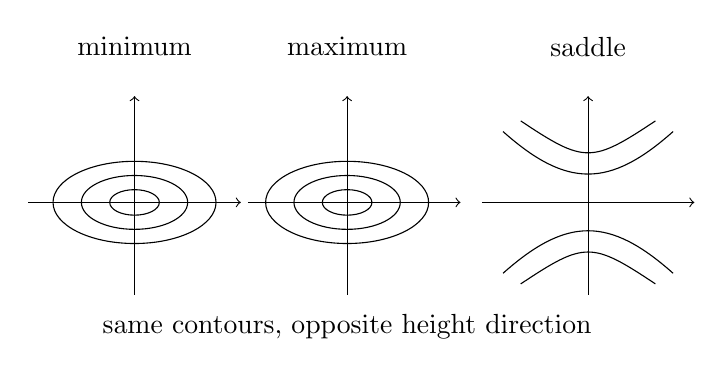
\begin{tikzpicture}[scale=0.9]
  \node at (-3,2.2) {minimum};
  \draw[->] (-4.5,0) -- (-1.5,0);
  \draw[->] (-3,-1.3) -- (-3,1.5);
  \draw (-3,0) ellipse (0.35 and 0.18);
  \draw (-3,0) ellipse (0.75 and 0.38);
  \draw (-3,0) ellipse (1.15 and 0.58);

  \node at (0,2.2) {maximum};
  \draw[->] (-1.4,0) -- (1.6,0);
  \draw[->] (0,-1.3) -- (0,1.5);
  \draw (0,0) ellipse (0.35 and 0.18);
  \draw (0,0) ellipse (0.75 and 0.38);
  \draw (0,0) ellipse (1.15 and 0.58);
  \node at (0,-1.75) {same contours, opposite height direction};

  \node at (3.4,2.2) {saddle};
  \draw[->] (1.9,0) -- (4.9,0);
  \draw[->] (3.4,-1.3) -- (3.4,1.5);
  \draw (2.2,-1.0) .. controls (3.1,-0.2) and (3.7,-0.2) .. (4.6,-1.0);
  \draw (2.2,1.0) .. controls (3.1,0.2) and (3.7,0.2) .. (4.6,1.0);
  \draw (2.45,-1.15) .. controls (3.35,-0.55) and (3.45,-0.55) .. (4.35,-1.15);
  \draw (2.45,1.15) .. controls (3.35,0.55) and (3.45,0.55) .. (4.35,1.15);
\end{tikzpicture}
\caption{Near a nondegenerate critical point, the Hessian determines the local quadratic shape.}
\end{figure}

\section{Constrained extrema}

Suppose one wants to optimize \(f(x,y)\) subject to a constraint
\[
  g(x,y)=0.
\]
At a regular point of the constraint curve, \(\nabla g\ne0\), so \(\nabla g\) is normal to the constraint.  At a constrained extremum, moving along the constraint produces no first-order change in \(f\).  Thus \(\nabla f\) must also be normal to the constraint.

\begin{theorem}[Lagrange multiplier condition]
If \(P_0\) is a constrained local extremum of \(f\) on \(g=0\), and \(\nabla g(P_0)\ne0\), then there exists \(\lambda\) such that
\[
  \nabla f(P_0)=\lambda\nabla g(P_0).
\]
\end{theorem}

For several constraints \(g_1=\cdots=g_k=0\), the gradient of \(f\) lies in the span of the constraint gradients:
\[
  \nabla f=\lambda_1\nabla g_1+\cdots+\lambda_k\nabla g_k.
\]

\begin{example}
Find extrema of \(f(x,y)=x+y\) on the circle \(x^2+y^2=1\).  The equations are
\[
  (1,1)=\lambda(2x,2y),
  \qquad x^2+y^2=1.
\]
Thus \(x=y\), and \(2x^2=1\), so
\[
  (x,y)=\left(\frac1{\sqrt2},\frac1{\sqrt2}\right)
  \quad\text{or}\quad
  (x,y)=\left(-\frac1{\sqrt2},-\frac1{\sqrt2}\right).
\]
The corresponding values are \(\sqrt2\) and \(-\sqrt2\), the maximum and minimum.
\end{example}

\section{Endpoint and boundary warnings}

The equation \(\nabla f=0\) applies only to interior unconstrained extrema.  The equation \(\nabla f=\lambda\nabla g\) applies only at regular constrained points.  If the domain has corners, endpoints, singular constraint points, or boundary pieces, they must be checked separately.

A reliable workflow is:
\[
\begin{array}{ll}
1. & \text{find interior critical points;}\\
2. & \text{find constrained or boundary candidates;}\\
3. & \text{check singular points and endpoints;}\\
4. & \text{compare values when the problem asks for absolute extrema.}
\end{array}
\]
